\documentclass{article}

% Please use the following line and do not change the style file.
\usepackage{icml2022_author_response}

% Recommended, but optional, packages for figures and better typesetting:
\usepackage{microtype}
\usepackage{graphicx}
\usepackage{subfigure}
\usepackage{hyperref}       % hyperlinks
\usepackage{booktabs} % for professional tables
\usepackage{amsfonts}       % blackboard math symbols
\usepackage{nicefrac}       % compact symbols for 1/2, etc.
\usepackage{xcolor}
\usepackage{lipsum}
\usepackage{wrapfig}

\begin{document}
% Uncomment the following line if you prefer a single-column format
\onecolumn

We sincerely appreciate all the reviewers for their valuable feedback  and nicely summarizing the highlights of our paper. In this rebuttal, we will answer the questions and provide some additional experiments as suggested. We hope our response can well address the concerns. Thank you.

{\color{blue} \textbf{Dear Reviewer \#1:}} \textbf{Literature:} Thanks for referring us to the series of interesting works. Yet, they are essentially different from ours. In [Belilovsky et. al, 2019], the model itself is trained in a layer-by-layer fashion by stacking shallow 1-layer networks, and [Ek et. al, 2020] and [Mo et. al, 2021] are applications of the above training strategy in different scenarios. However, in our approach, the model is trained in the standard federated learning framework (all layers at the same time), with adaptive AMSGrad as the local optimizer, and layer-wise adaptive learning rates. To the best of our knowledge, applying local layer-wise learning rate adjustment to FL has not been studied before. We will cite the mentioned papers and clarify the differences as suggested. Thank you.


\textbf{Experiments:} adf asdfasfasdfafasdfasfd as f

\begin{wrapfigure}{r}{0.25\textwidth}
  \begin{center}
  \vspace{-0.25in}
    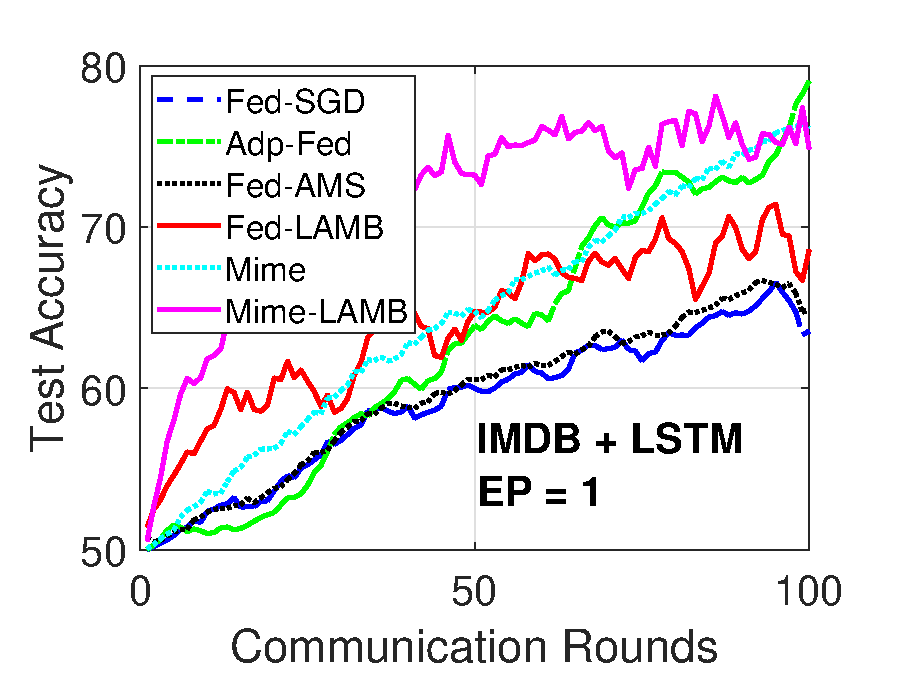
\includegraphics[width=1.8in]{icml_rebuttal_fig/imdb_testerror_lstm_ep1_client50_iid0.eps}
  \end{center}
  \vspace{-0.15in}
  \caption{IMDB + LSTM, non-IID.}
  \label{emp-var}\vspace{-0.1in}
\end{wrapfigure}


\textbf{Insight:} The insight of the layer-wise adaptive learning rate is that in NN, the magnitude of layer weights and gradients might differ a lot. If the gradient (of a layer) is too small, the weight will not move sufficiently far which slows down the convergence. Thus, besides the coordinate-wise adaptivity brought by local AMSGrad, we further incorporate the layer-wise adaptivity to adjust the learning rates layer-by-layer in every training iteration. The results show that our method can achieve faster convergence, also with possibly improved accuracy, in both IID and non-IID settings. The improved convergence also implies reduced communication cost, since the model needs fewer rounds to converge.

\textbf{Extension:} Yes, we believe our idea of adopting layer-wise learning rates in FL can be extended to many other methods, such as local SGD and SGD with momentum. Meanwhile, it may also be applied to the adaptive central server updates in FL (e.g., the Adp-Fed method, Algorithm 2 in Appendix A). These are all possible future directions.

\begin{wrapfigure}{r}{0.3\textwidth}
  \begin{center}
  \vspace{-0.25in}
    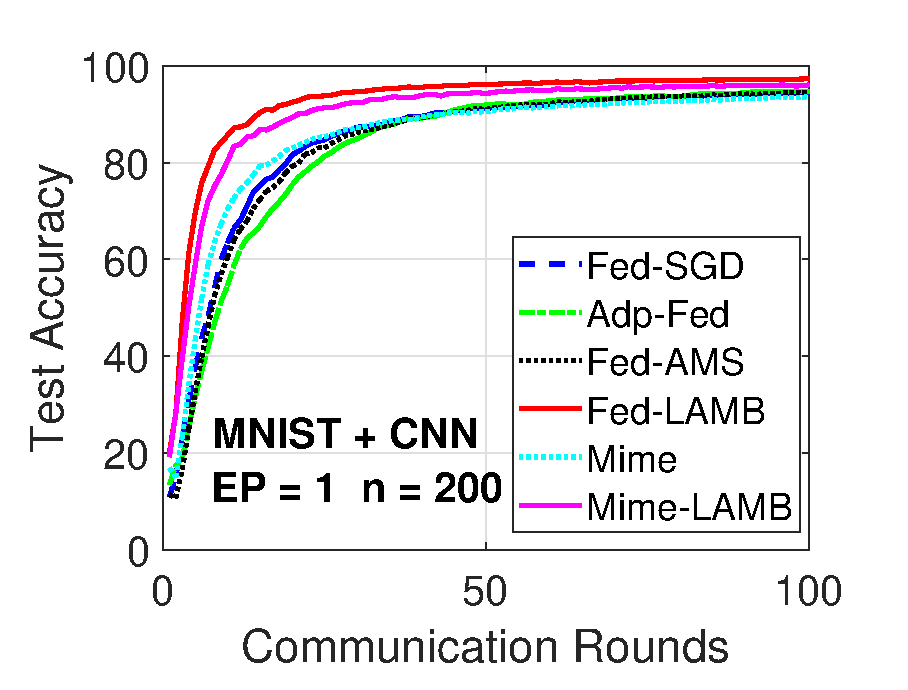
\includegraphics[width=1.4in]{icml_rebuttal_fig/mnist_testerror_cnn_ep1_client200_iid0.eps}
    % 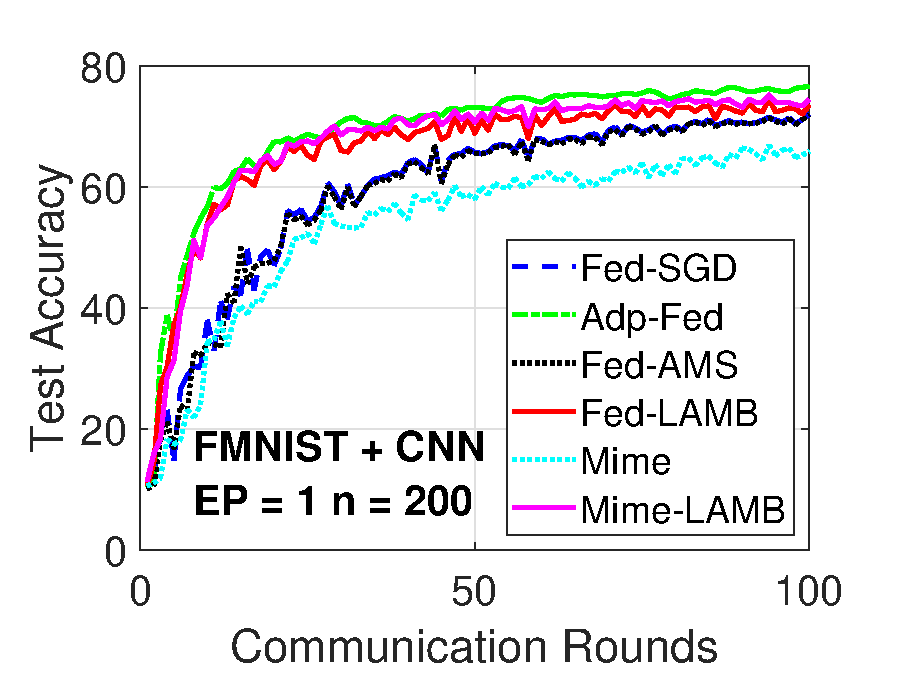
\includegraphics[width=1.4in]{icml_rebuttal_fig/fmnist_testerror_cnn_ep1_client200_iid0.eps}
  \end{center}
  \vspace{-0.15in}
  \caption{IMDB + LSTM, non-IID.}
  \label{emp-var}\vspace{-0.1in}
\end{wrapfigure}

\begin{wrapfigure}{r}{0.25\textwidth}
  \begin{center}
  \vspace{-0.25in}
    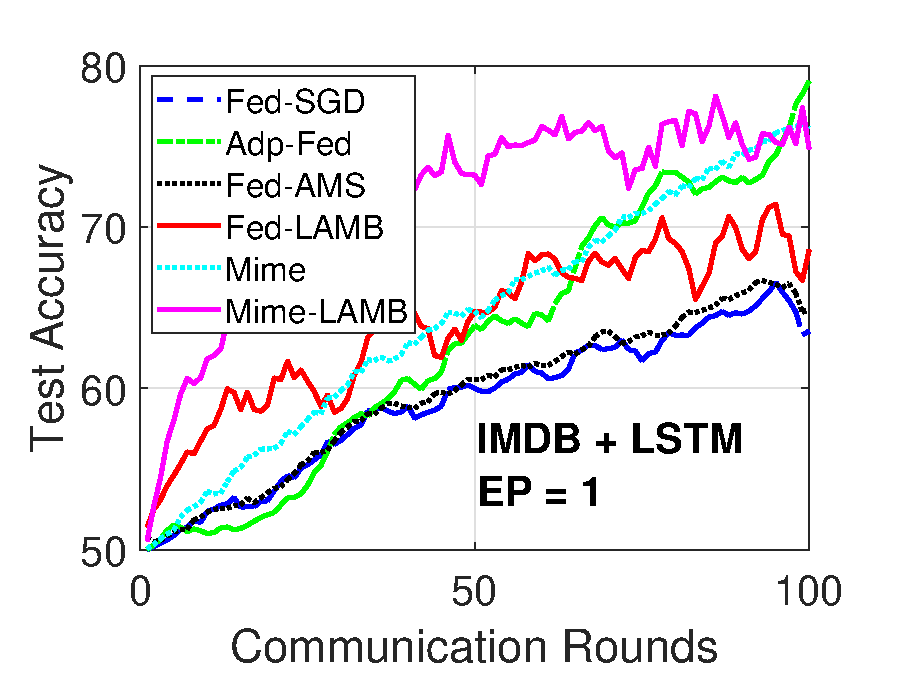
\includegraphics[width=1.8in]{icml_rebuttal_fig/imdb_testerror_lstm_ep1_client50_iid0.eps}
  \end{center}
  \vspace{-0.15in}
  \caption{IMDB + LSTM, non-IID.}
  \label{emp-var}\vspace{-0.1in}
\end{wrapfigure}

{\color{blue} \textbf{Dear Reviewer \#4:}} \textbf{Novelty of algorithm and theory:} Thanks for mentioning [Charles et. al, NeurIPS 2021], which will be discussed in the paper. Note that, Charles et. al apply layer-wise adaptivity at the central server with local updates still using SGD. This is exactly the Adp-Fed method (Alg. 2 in Appendix A) + LAMB at central node. Our approach is essentially different, since it is built upon local adaptive methods, where local updates follow AMSGrad and layer-wise adaptivity is applied at local models. Also, Charles et. al only provides empirical results, while we also give the convergence analysis. Regarding the convergence rate, note that while in [You et. al, 2020] LAMB shows considerable empirical improvement over Adam, theoretically, the convergence rate of LAMB is the same as that of Adam under common assumptions. In our paper, we show that the convergence rate of Fed-LAMB can also match that of Fed-AMS, in the FL setting. To our knowledge, this is the first convergence analysis of layer-wise adaptive strategy in FL. Therefore, we believe that our algorithm design and theoretical analysis could provide novel contribution to the community.



{\color{blue} \textbf{Dear Reviewer \#4:}} \textbf{Second moment aggregation:} In the original paper of [Li et. al, 2020] and [Karimireddy et. al, 2020], the authors have shown that the performance of Fed-AMS and Mime would be much worse without sharing $v$. Since $v$ controls the implicit learning rate for every dimension, synchronizing $v$ makes all the clients ``on the same pace'' which helps convergence. Thus, at this stage, the synchronization of $v$ seems a necessary part in the design of federated adaptive methods. One possible trick in practice is to reduce the frequency of communicating $v$. This can reduce the extra communication cost of $v$, without affecting the theoretical convergence rate.

\textbf{Maximum operator:} Yes, in practice, we found that ignoring the maximum operation at the central server gives similar results. Since it is known that the theoretical convergence of Adam (without the max) could be problematic, we use AMSGrad (with the max) as the backbone algorithm for soundness, which is also implemented in our experiments for consistency.

\end{document}
